\documentclass[a4paper,12pt]{article}
%report, book

%отступы
\usepackage[left=1cm,right=1cm,top=1cm,bottom=2cm,bindingoffset=0cm]{geometry}
\usepackage{indentfirst}

%Рисунки
\usepackage{graphicx}
\usepackage{wrapfig}

%Ссылки
\usepackage{hyperref}
\usepackage[rgb]{xcolor}
\hypersetup{
    colorlinks=true,
    urlcolor=blue
}

%Русский язык
\usepackage[T2A]{fontenc}
\usepackage[utf8]{inputenc}
\usepackage[english,russian]{babel}

%Математика
\usepackage{amsmath,amsfonts,amssymb,amsthm,mathtools}
\usepackage{icomma}

%Доп пакеты
\usepackage{subcaption}
\usepackage{ upgreek }
\usepackage{float}


\usepackage{listings}
\usepackage{xcolor}

\definecolor{codegreen}{rgb}{0,0.6,0}
\definecolor{codegray}{rgb}{0.5,0.5,0.5}
\definecolor{codepurple}{rgb}{0.58,0,0.82}
\definecolor{backcolour}{rgb}{0.95,0.95,0.92}

\lstdefinestyle{mystyle}{
    backgroundcolor=\color{backcolour},   
    commentstyle=\color{codegreen},
    keywordstyle=\color{magenta},
    numberstyle=\tiny\color{codegray},
    stringstyle=\color{codepurple},
    basicstyle=\ttfamily\footnotesize,
    breakatwhitespace=false,         
    breaklines=true,                 
    captionpos=b,                    
    keepspaces=true,                 
    numbers=left,                    
    numbersep=5pt,                  
    showspaces=false,                
    showstringspaces=false,
    showtabs=false,                  
    tabsize=2
}

\lstset{style=mystyle}



%Чтобы найти символ, используем Detexify -> https://detexify.kirelabs.org/classify.html
%Для перевода excel->latex используем Tables Generator -> https://www.tablesgenerator.com/latex_tables
%Для распознования текста по картинке -> https://img2txt.com/ru
%Небольшой тутор по графикам -> http://cs.mipt.ru/python/lessons/lab1.html
%Также -> https://stackoverflow.com/questions/2409774/how-can-i-produce-student-style-graphs-using-matplotlib

%Заголовок
\author{Финоченко Александр}
\title{}
\date{\today}

\begin{document}
\begin{center}
\Large{
\textbf{Лабораторная работа 1}

\textbf{Асимптотическая сложность}

Финоченко Александр Викторович Б02-201
}

\end{center}
\large

\textbf{Цель работы:} проверить прямыми измерениями времени асимптотическую сложность алгоритмов по времени в зависимости от объёма данных.


\section*{Поиск}

\subsection*{Полный перебор (папка exhaustive\_search)}
Сначала было измерено время для полного перебора (папка exhaustive\_search). Для каждого $N$ сразу в программе находилось среднее время для 1000 измерений.

Код функции полного перебора:
\begin{lstlisting}[language=C++]
int exhaustive_search(int* A, int N, int value) {
	for (int i = 0; i < N; i++) {
		if (A[i] == value)
			return i;
	}
	return -1;
}
\end{lstlisting}


Чтобы построить график воспользуемся МНК. Если график представим в виде $t = aN+b$, то по МНК
\begin{center}
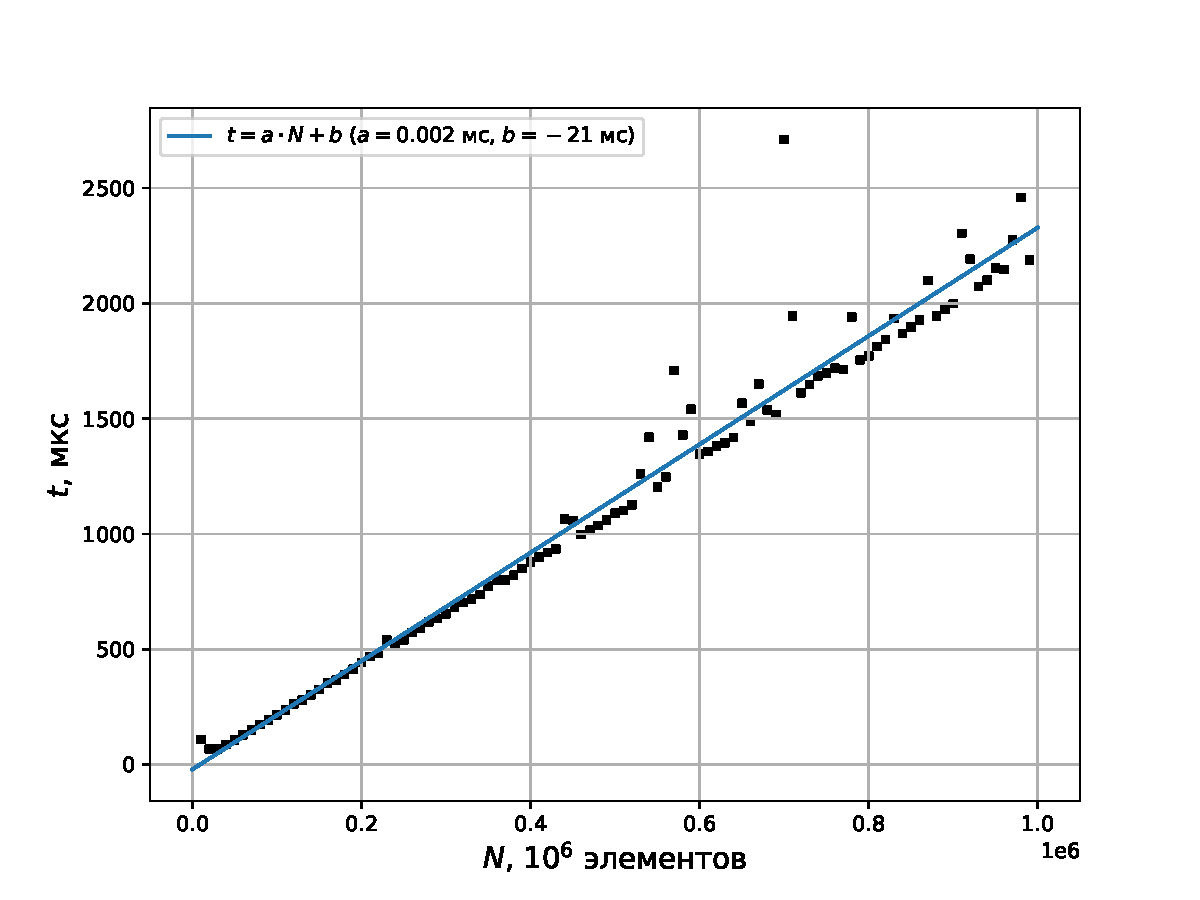
\includegraphics[scale=0.8]{Figure_1.pdf}
\end{center}

Получаем хорошую линейную зависимость времени от объёма данных.


\subsection*{Бинарный поиск (папка binary\_search)}
Для измерения использовалась программа из папки binary\_search. При малом количестве повторений программа выдавала сильно разные значения времени, поэтому было выбрано делать для одного $N$ 100000000 измерений в одной программе.

Код функции бинарного поиска имеет вид
\begin{lstlisting}[language=C++]
int binary_search(int* A, int N, int value) {
	int a = 0, b = N - 1, mid;
	bool flag = false;
	while ((a <= b) && (flag == false)) {
		mid = (a + b) / 2;
		if (A[mid] == value) return mid;
		if (A[mid] > value) b = mid - 1;
		else a = mid + 1;
	}
	return -1;
}
\end{lstlisting}



Если график представим в виде $t = a \log_2 N + b$,  то по МНК


\begin{center}
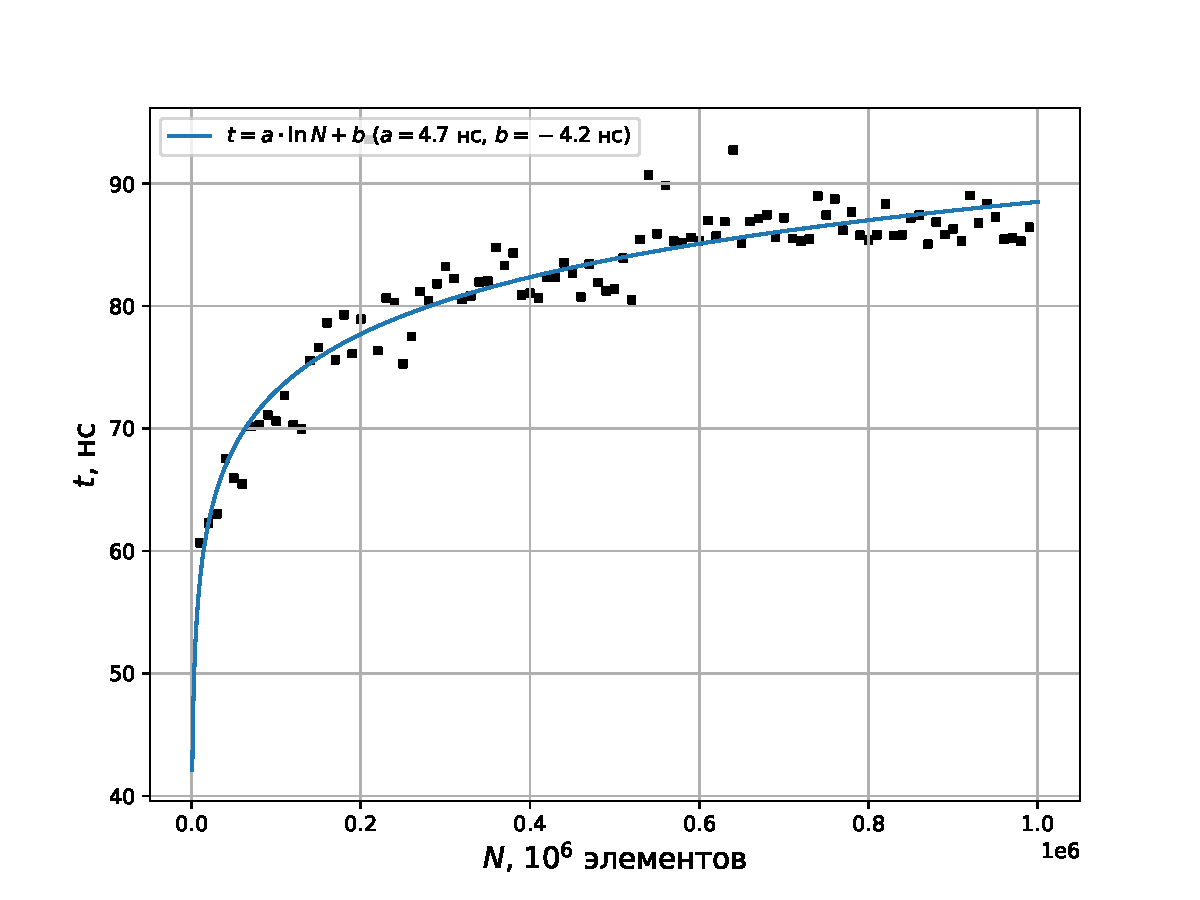
\includegraphics[scale=1]{Figure_2.pdf}
\end{center}

Получаем нормальную логарифмическую зависимость времени от объёма данных.

\section*{Сумма двух}

\subsection*{Полный перебор $O(N^2)$ (папка sum\_of\_two)}
Было измерено время для полного перебора с вложенным циклом . Для каждого $N$ сразу в программе находилось среднее время для 1000 измерений.

Код функции полного перебора представлен ниже
\begin{lstlisting}[language=C++]
void sum_search(int* A, int N, int value) {
	for (int i = 0; i < N - 1; i++) {
		for (int j = i + 1; j < N; j++) {
			if (A[i] + A[j] == value) {
				cout << i << " " << j << "\n";
				return;
			}
		}
	}
}
\end{lstlisting}

Если график представим в виде $t = a \log_2 N + b$,  то по МНК $a = 7.47 \cdot 10^{-7}$ мс, $b = 1 \cdot 10^{-5}$ мс, $c = -4.8 \cdot 10^{-2}$ мс.

\begin{center}
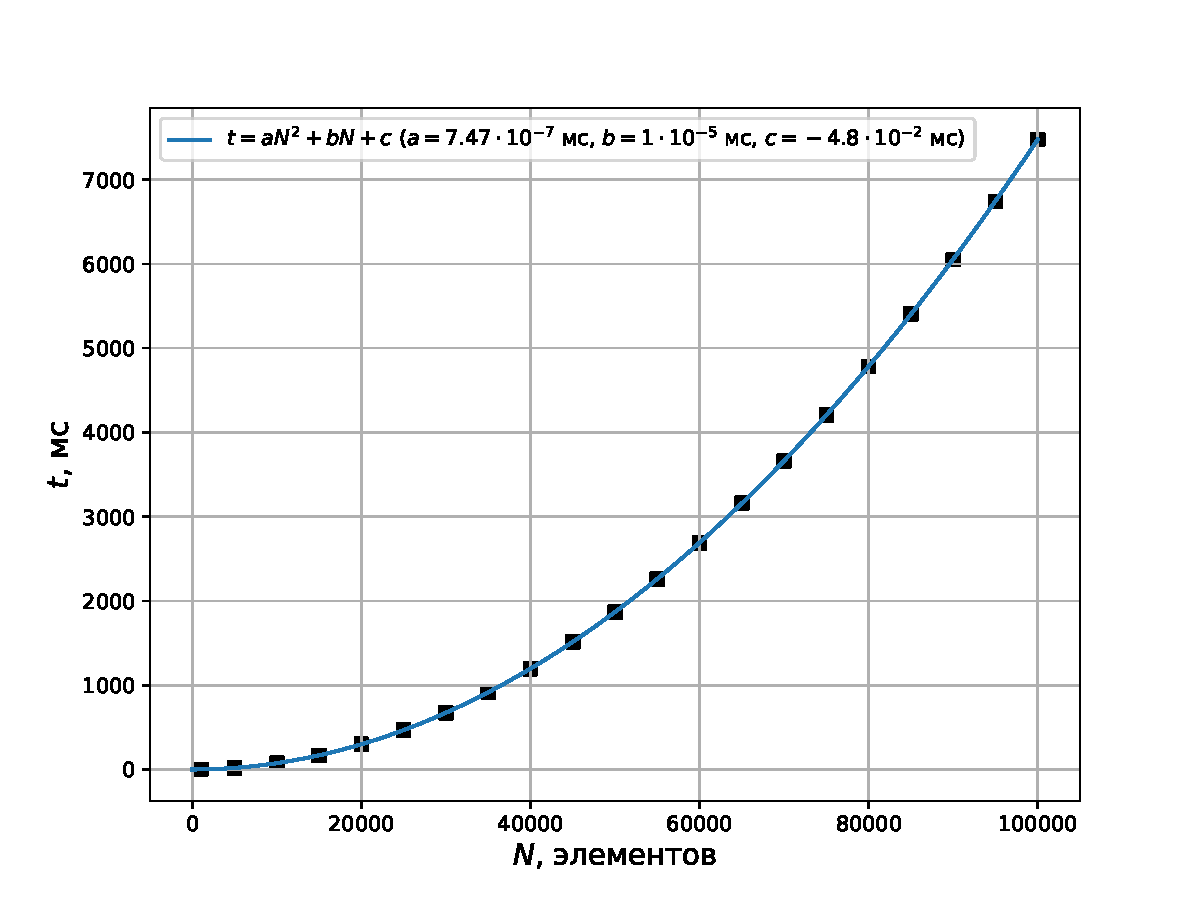
\includegraphics[scale=1]{Figure_3.pdf}
\end{center}

Получаем хорошую квадратичную зависимость времени от объёма данных.

\subsection*{Алгоритм поиска $O(N)$ (папка sum\_ON)}

Код функции, работающей по алгоритму с асимптотикой $O(N)$, представлен ниже

\begin{lstlisting}[language=C++]
void sum_of_two(int* A, int N, int value) {
	int i = 0, j = N - 1;
	while (i != j) {
		if (A[i] + A[j] == value) {
			cout << i << " " << j << "\n";
			return;
		}
		if (A[i] + A[j] > value)
			j--;
		else
			i++;
	}
}
\end{lstlisting}

Берутся два крайних индекса, если сумма значений больше, то уменьшаем верхний индекс, меньше -- увеличиваем нижний, если равна -- выводим значения.Заметим, что этот алгоритм корректно работает. Для каждого $N$ сразу в программе находилось среднее время для 1000 измерений.


Чтобы построить график воспользуемся МНК. Если график представим в виде $t = aN+b$, то по МНК

\begin{center}
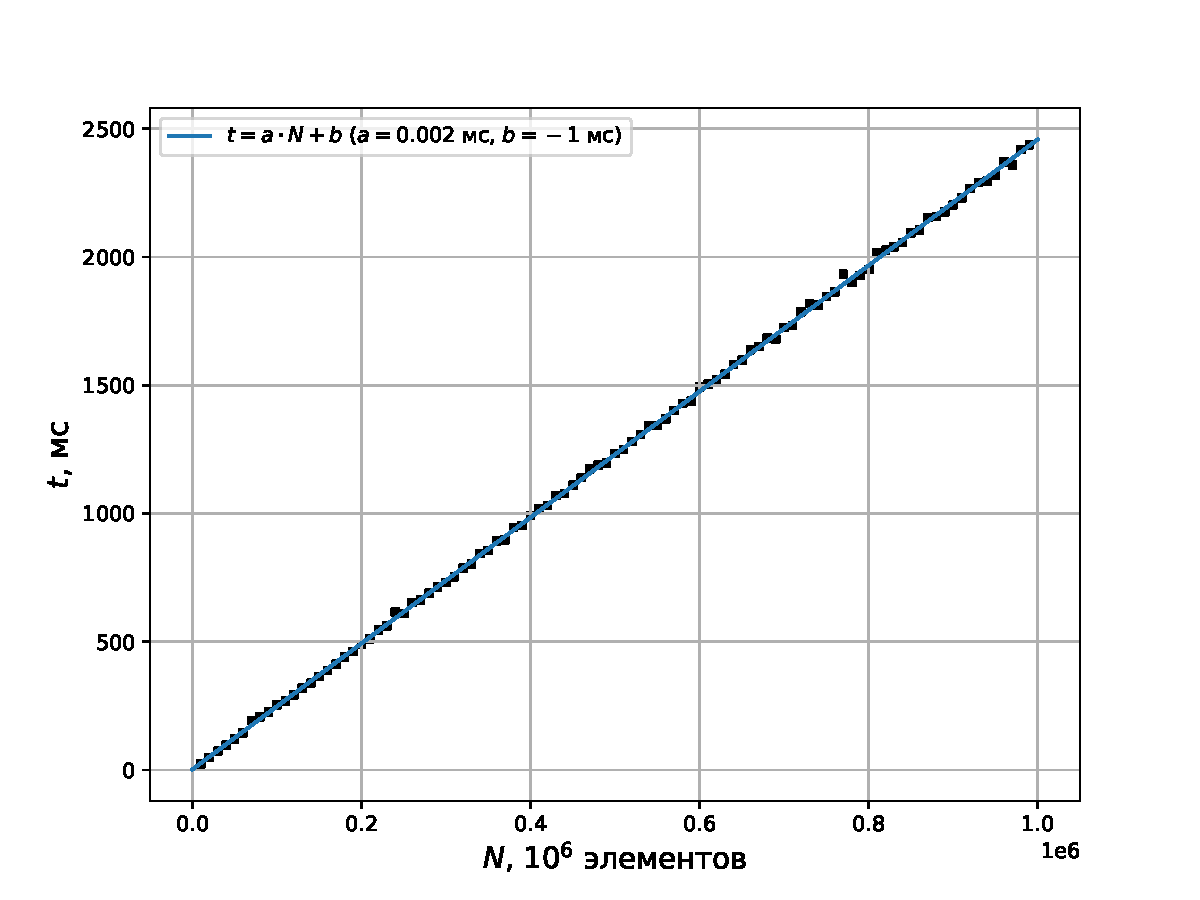
\includegraphics[scale=0.8]{Figure_4.pdf}
\end{center}

\section*{Часто используемый элемент}
Приведем три стратегии

\begin{lstlisting}[language=C++]
void strategy_A(int* A, int N) {
	for (int i = 1; i < N; i++) {
		if (A[i] != A[0]) {
			int temp;
			temp = A[0];
			A[0] = A[i];
			A[i] = temp;
		}
	}
}
\end{lstlisting}

\begin{lstlisting}[language=C++]
void strategy_B(int* A, int N) {
	for (int i = 1; i < N; i++) {
		if (A[i] != A[0]) {
			int temp;
			temp = A[i-1];
			A[i-1] = A[i];
			A[i] = temp;
		}
	}
}
\end{lstlisting}

\begin{lstlisting}[language=C++]
void strategy_C(int* A, int N) {
	int carr[MAX_RAND + 1] = {0};
	for (int i = 0; i < N; i++) {
		carr[A[i]]++;
	}
	for (int i = 1; i < N; i++) {
		if (carr[A[i]] > carr[A[i - 1]]) {
			int temp = A[i - 1];
			A[i - 1] = A[i];
			A[i] = temp;
		}
	}
}
\end{lstlisting}

\subsection*{Равномерный массив}
Равномерный массив был создан просто как последовательность чисел от 1 до $N$. Т.к. у равномерного массива все числа встречаются 1 раз, то для поиска было выбрано случайное число.

Приведём графики

\begin{center}
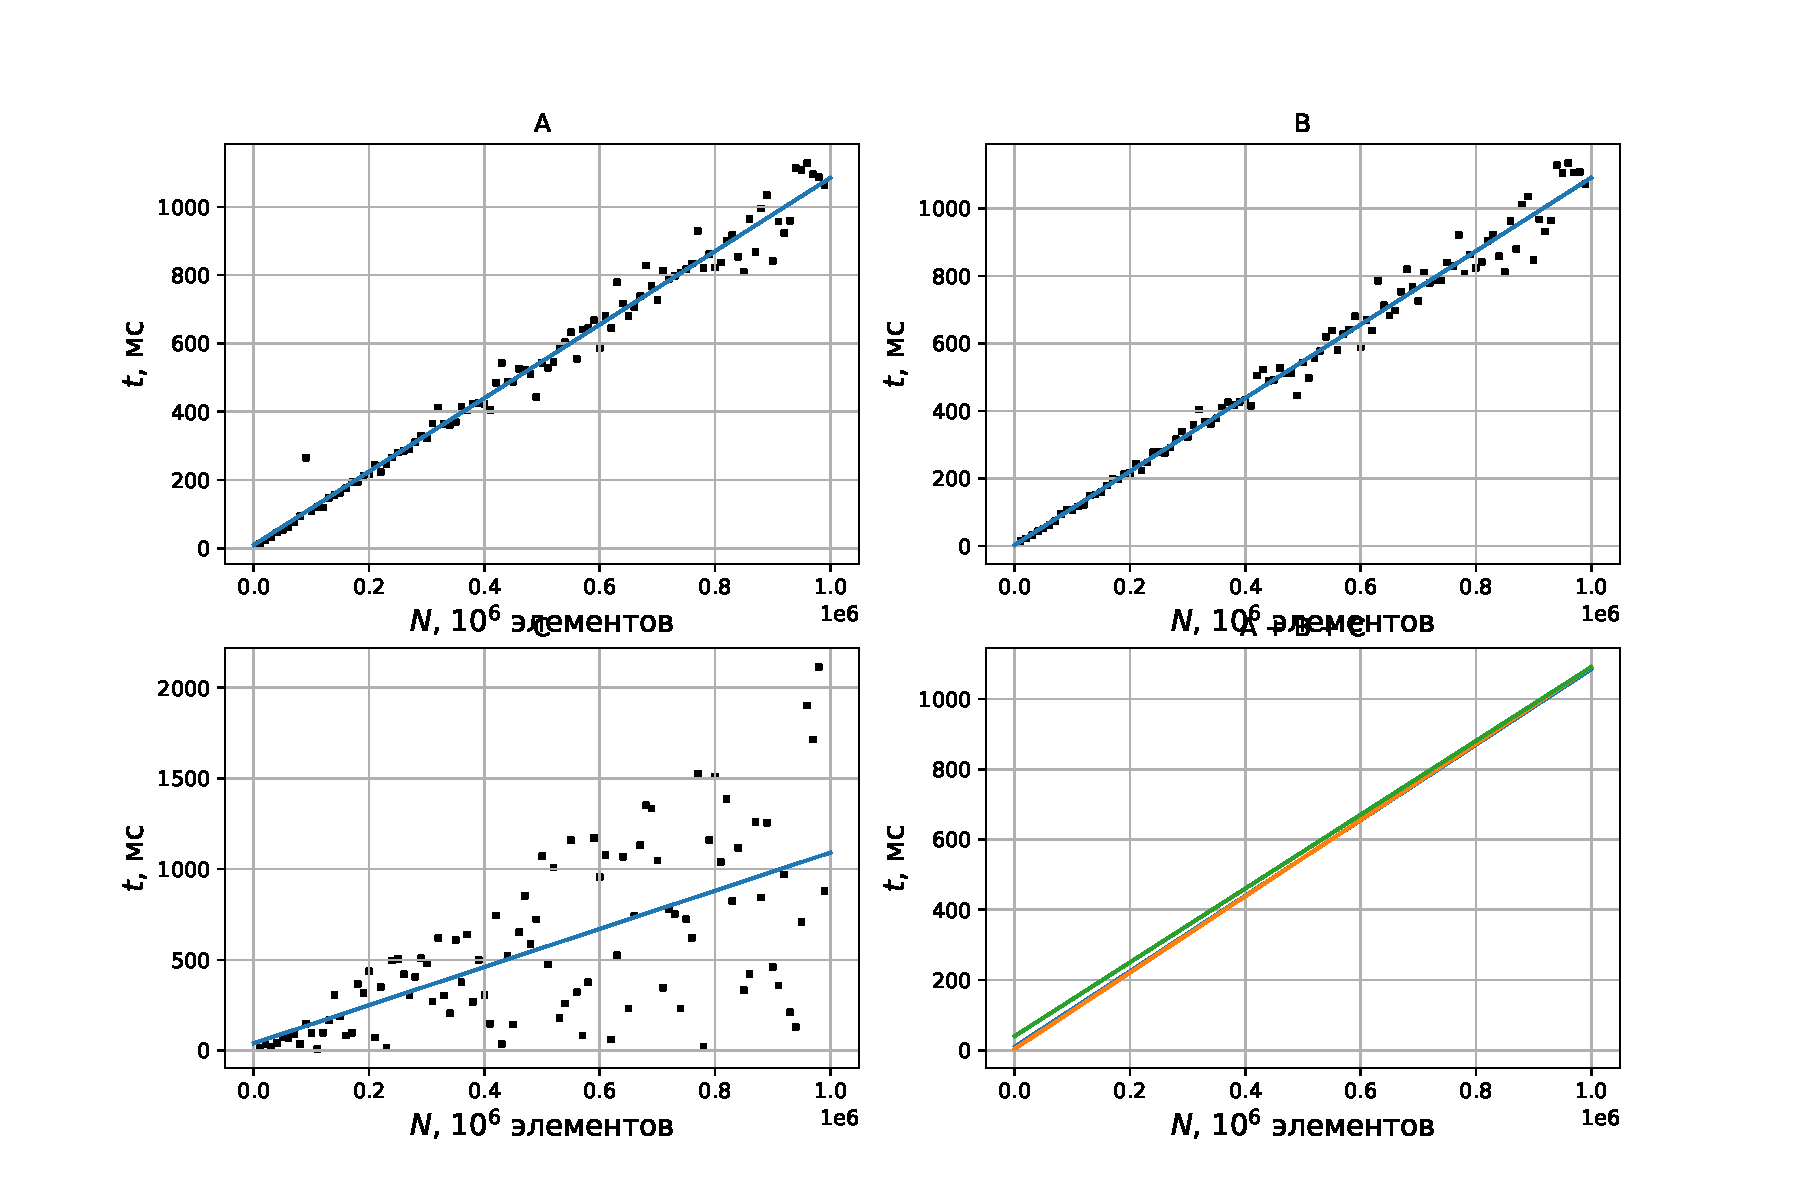
\includegraphics[scale=0.5]{Figure_5.pdf}
\end{center}

Видно, что асимптотика не зависит от стратегии.

\subsection*{Неравномерный массив}
Неравномерный массив был создан просто как случайных чисел от 1 до $MAX_RAND$. Т.к. у неравномерного массива числа могут встретиться несколько раз, для поиска выбирается наиболее распространенное число число.

Приведём графики

\begin{center}
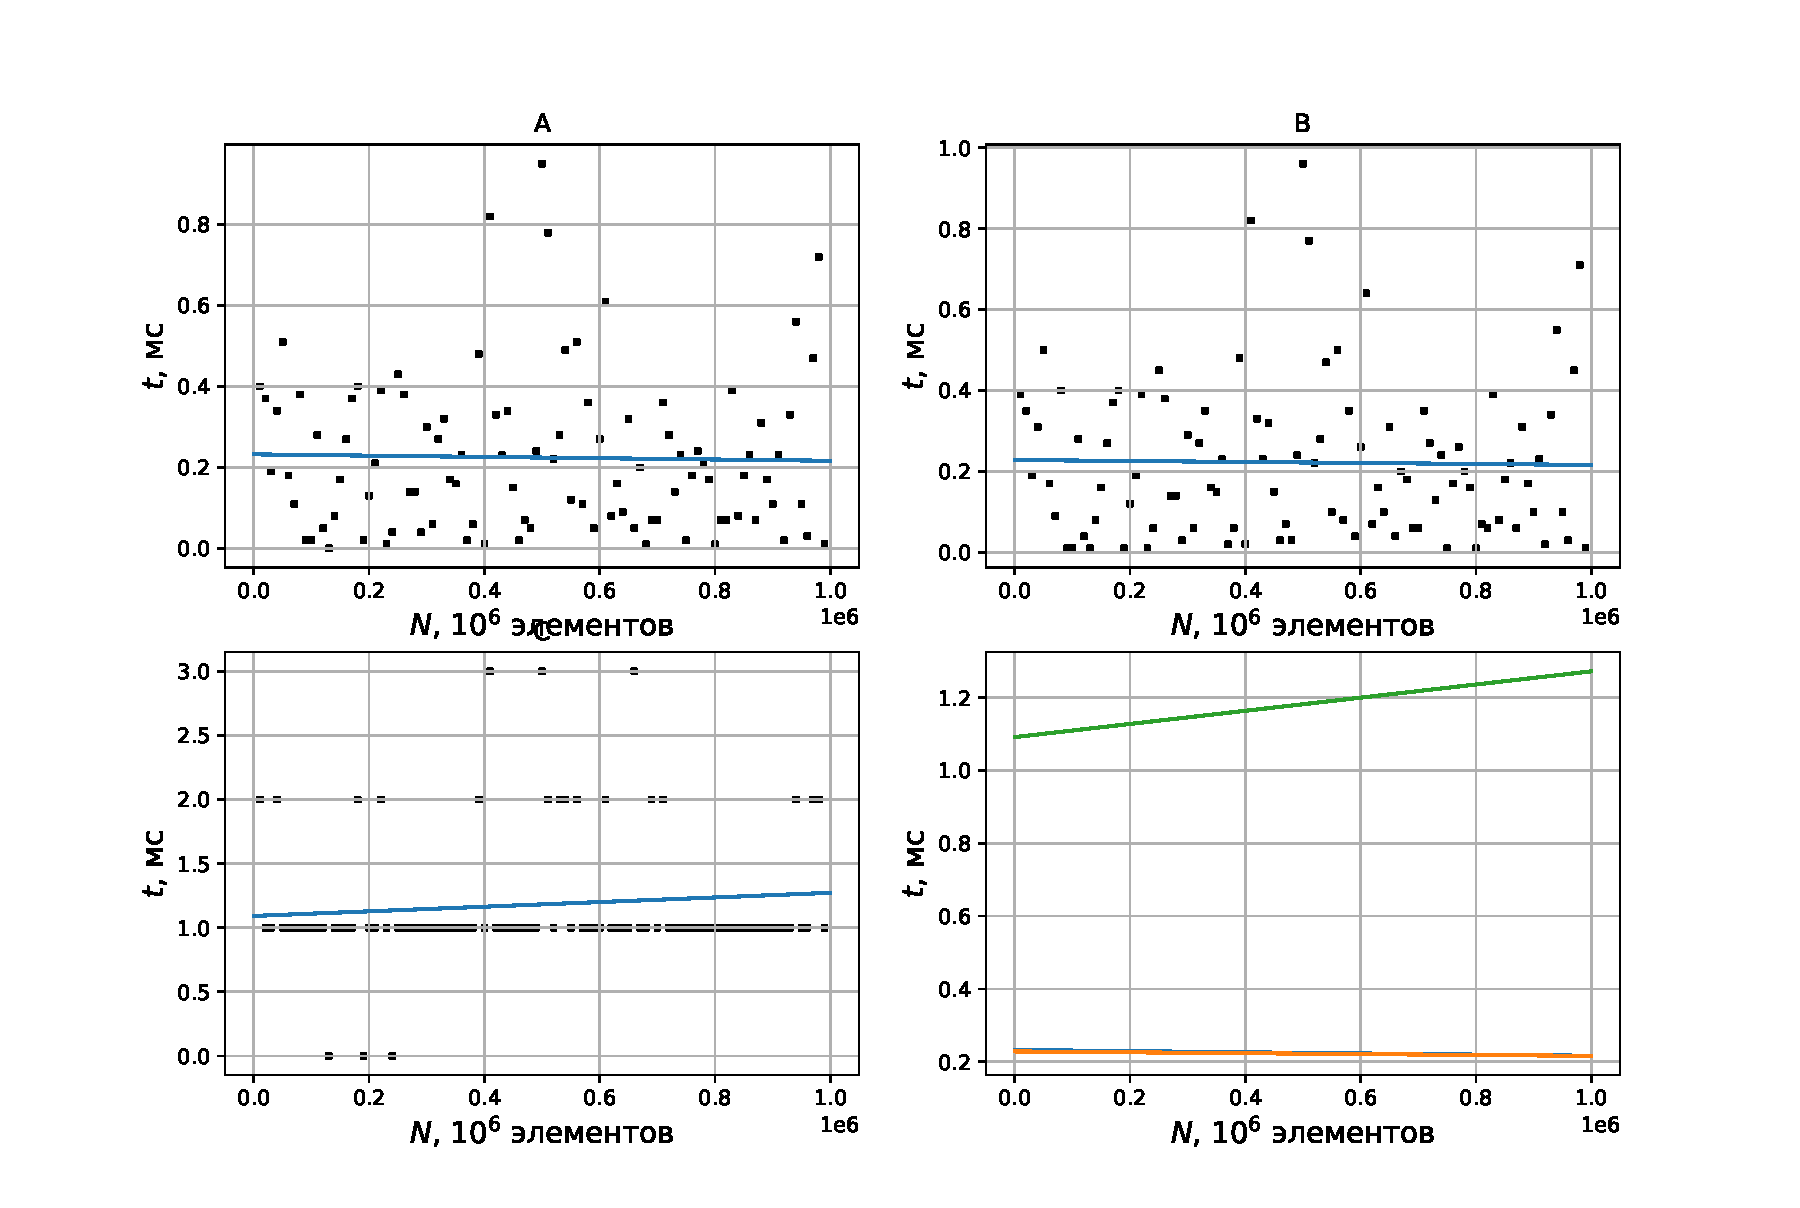
\includegraphics[scale=0.5]{Figure_6.pdf}
\end{center}

Видим, что стратегии A и B дают асимптотику $O(1)$. Стратегия C всё равно даёт $O(N)$.

\end{document}
